%%%%%%%%%%%%%%%%%%%%%%%%%%%%%%%%%%%%%%%%%%%%%%%%%%%%%%%%%%%%%%%%%%%%%
%
%  This is a sample LaTeX input file for your contribution to 
%  the MC2013 conference. Modified by R.C. Martineau at INL from A. 
%  Sood at LANL, from J. Wagner ORNL who obtained the original class 
%  file by Jim Warsa, LANL, 16 July 2002}
%
%  Please use it as a template for your full paper 
%    Accompanying/related file(s) include: 
%       1. Document class/format file: mc2013.cls
%       2. Sample Postscript Figure:   figure.eps
%       3. A PDF file showing the desired appearance: template.pdf 
%    Direct questions about these files to: richard.martinea@inl.gov
%
%    Notes: 
%      (1) You can use the "dvips" utility to convert .dvi 
%          files to PostScript.  Then, use either Acrobat 
%          Distiller or "ps2pdf" to convert to PDF format. 
%      (2) Different versions of LaTeX have been observed to 
%          shift the page down, causing improper margins.
%          If this occurs, adjust the "topmargin" value in the
%          mc2013.cls file to achieve the proper margins. 
%
%%%%%%%%%%%%%%%%%%%%%%%%%%%%%%%%%%%%%%%%%%%%%%%%%%%%%%%%%%%%%%%%%%%%%


%%%%%%%%%%%%%%%%%%%%%%%%%%%%%%%%%%%%%%%%%%%%%%%%%%%%%%%%%%%%%%%%%%%%%
\documentclass{mc2013}
%
%  various packages that you may wish to activate for usage 
\usepackage{graphicx}
\usepackage{tabls}
\usepackage{afterpage}
\usepackage{cites}
\usepackage{color}
\usepackage{amsmath,amsthm,amssymb}
\usepackage{verbatim}
\usepackage[parfill]{parskip}
\usepackage{tikz}
 
\newcommand{\N}{\mathbb{N}}
\newcommand{\Z}{\mathbb{Z}}
\newcommand{\deriv}[2]{\frac{\mathrm{d} #1}{\mathrm{d} #2}}
\newcommand{\pderiv}[2]{\frac{\partial #1}{\partial #2}}
\newcommand{\bx}{\mathbf{X}}
\newcommand{\ba}{\mathbf{A}}
\newcommand{\by}{\mathbf{Y}}
\newcommand{\bj}{\mathbf{J}}
\newcommand{\bs}{\mathbf{s}}
\newcommand{\B}[1]{\ensuremath{\mathbf{#1}}}
\newcommand{\Dt}{\Delta t}
\renewcommand{\d}{\mathrm{d}}
\newcommand{\mom}[1]{\langle #1 \rangle}
\newcommand{\xl}{{x_{i-1/2}}}
\newcommand{\xr}{{x_{i+1/2}}}
\newcommand{\il}{{i-1/2}}
\newcommand{\ir}{{i+1/2}}

\graphicspath{{figures/}}
 
%\usepackage{epsf}
%
%
% Insert authors' names and short version of title in lines below
%
\newcommand{\authorHead}      % Author's names here
   {Authors' names, use et al. if more than 3}  
\newcommand{\shortTitle}      % Short title here
   {Short version of title as entered by author on web page}  
%%%%%%%%%%%%%%%%%%%%%%%%%%%%%%%%%%%%%%%%%%%%%%%%%%%%%%%%%%%%%%%%%%%%%
%
%   BEGIN DOCUMENT
%
%%%%%%%%%%%%%%%%%%%%%%%%%%%%%%%%%%%%%%%%%%%%%%%%%%%%%%%%%%%%%%%%%%%%%
\begin{document}

%
%      Headers and Footers
\afterpage{%
\fancyhf{}%
\fancyhead[CE]{              
{\scriptsize \authorHead}}                                                
\fancyhead[CO]{               
{\scriptsize \shortTitle}}                  
%\lfoot{\scriptsize{
%International Conference on Mathematics and Computational Methods
%Applied to Nuclear Science \& Engineering (M\&C 2013), 
%\\ Sun Valley, Idaho, USA, May 5-9, 2013.}}%
\rfoot{\thepage/\totalpages{}}%

\pagestyle{fancy}
%\setlength{\topmargin}{-20pt}
}
 
\normalsize

\setlength{\baselineskip}{16.8pt}
\vspace{-3pt}

% 
% TITLE
%

\begin{center}
\textbf{\large \\%
A HIGH-ORDER LOW-ORDER ALGORITHM WITH EXPONENTIALLY-CONVERGENT MONTE CARLO FOR
THERMAL RADIATIVE TRANSFER\\
}
% 
% FIRST AUTHORS 
%
\setlength{\baselineskip}{14pt}
\textbf{S.R. Bolding and J.E. Morel} \\
Department of Nuclear Engineering\\
Texas A\&M University  \\
College Station, TX 77843 \\
sbolding@tamu.edu; morel@tamu.edu \\

% 
% SECOND AUTHORS (if not needed delete from here) 
%
\vspace{12pt}
\textbf{Double space and list Author C}\\
Department of Nuclear Engineering  \\
Name of University \\
Address \\
C@name.univ.edu\\ 
%
% SECOND AUTHORS (to here)
%

\end{center}

%
% SET RAGGED RIGHT MARGIN
%
\raggedright


\section*{ABSTRACT} 
\begin{quote}
\begin{small}
We have demonstrated the potential of a new high-order low-order (HOLO) algorithm for solving
thermal radiative transfer problems.  The low-order (LO) solver is based on spatial
and angular moments of the transport equation and a linear discontinuous
finite-element spatial representation.  
The LO solver is fully implicit in time and resolves the non-linear
temperature dependence at each time step.  The solution to the LO solver produces a
fixed-source, pure absorber transport problem as the high-order (HO) system.  The HO solver
utilizes exponentially-convergent Monte Carlo (ECMC) to give a globally accurate solution
for the angular intensity.  This global solution is used to compute consistency terms
that require the HO and LO solutions to converge to the same solution.  The use of ECMC
eliminates instabilities caused by statistical noise introduced to the LO consistency
terms.  Herein, we discuss the method in detail and compare initial results with an
implicit Monte Carlo code for one-dimensional gray test problems.
\emph{Key Words}: List of at most five key words

\end{small} 
\end{quote}

\setlength{\baselineskip}{14pt}
\normalsize

\Section{INTRODUCTION}

Thermal radiative transfer (TRT) physics are relevant in many high-temperature physical applications,
e.g., inertial confinement fusion and supernovae.  Such problems feature a strong
coupling between between the material and radiation energy balance equations, as well
as non-linear material and source term temperature dependences.  TRT problems often require solutions in a mix of
streaming and diffusive regions of the problem due to absorption-reemission physics
and opacity temperature dependencies. The diffusive regions are time
consuming to solve with higher-rank transport solutions and can be accurately
represented by a diffusion solution.  However, streaming regions require the accuracy of
a full transport treatment. 

Moment-based hybrid Monte Carlo (MC) methods have been proven useful for solving
non-linear, TRT problems. Recent work has focused on fixed-point iteration high-order low-order
(HOLO) approaches~\cite{willert,park,rmc}.   Such methods utilize a low-order (LO) operator based on angular moments of the
transport equation, formulated over a coarse spatial mesh.
Physics operators that are time
consuming for the HO transport solver to resolve, e.g., the re-emission source and
physical scattering, are moved to the LO system.  
Newton methods allow for non-linearities in the LO equations to
be efficiently solved~\cite{willert}. This allows for non-linear
terms at each time step to be accurately resolved, eleminating the need for
approximate linearizations and short time steps relevant to other methods.

High-fidelity solutions can be achieved with HOLO methods by using standard
MC simulations to solve the HO transport
equation. The HO solution is used to construct consistency
terms that require the LO solution to be consistent with the HO solution.  These
consistency terms preserve
the accuracy of the MC solution method in the LO operator. Such HOLO algorithms suffer from stability issues caused by statistical noise introduced into the
consistency terms that are estimated via MC simulation.  
In this work, we demonstrate the utility of a unique LO operator in conjunction with
an exponentially-convergent Monte
Carlo (ECMC) method\cite{jake} for the HO solver.  The ECMC algorithm
allows for statistical noise to be reduced to the same order as the HOLO iteration
error with significantly less particles than standard MC. We have derived the LO operator
directly from the transport equation, using a linear-discontinuous (LD)
finite-element (FE) spatial
discretization, such that the
HO and LO solutions are consistent upon convergence. The LD spatial representation
mitigates issues with energy propagating faster than the speed of light by providing an
accurate spatial representation of the Planckian emission term within a cell.  We
present results for various Marshak wave test problems and reference are results
against IMC.

\Section{High-Order Low-Order Algorithm for Thermal Radiative Transfer}

\Subsection{Governing Equations} 

We have implemented a high-order low-order (HOLO) algorithm for the case of gray, one spatial dimension
TRT problems. For simplicity, we will also consider constant density and specific
heats throughout.  The governing equations are the radiation and
material energy balance equations, i.e.,
\begin{align}
    \frac{1}{c}\pderiv{I}{t} + \mu \pderiv{I}{x} + \sigma_t I
&= \frac{\sigma_s}{2} \phi +\frac{1}{2} \sigma_a a c T^4
  \\
  \rho c_v \pderiv{T}{t} &= \int_{-1}^{1} \sigma_a I^{n+1}(x,\mu)
\d\mu - \sigma_a a c (T^4),
\end{align}
where $\phi(x) = \int_{-1}^1 I(x,\mu) \d \mu$ is the scalar radiation intensity,
related to the energy density $E(x)=\phi(x)/c$. Here, $x$ is the position,  $\mu$ is
the $x$-direction cosine, and $a$, $c$, $\rho$, $c_v$, $\sigma_a$, $\sigma_s$, and
$\sigma_t$ are the radiation constant, speed of light, mass density, specific heat, absorption, scattering, and total
opacities (cm$^{-1}$), respectively.  The desired fundamental unknowns are the material
temperature $T(x)$ and radiation intensity $I(x,\mu)$.  In general, the material
properties are a function of $T$.
The equations are coupled through the gray Planckian emission source
$\sigma_a a c T^4$ and absorption term $\sigma_a \phi$.  
The notation of the scalar intensity $\phi$ is used throughout rather than the
typical radiation energy density $E=\phi(x)/c$.

MC solution to the TRT equations is typically achieved by the well-known
implicit Monte Carlo (IMC) method, first introduced by Fleck and Cummings~\cite{fnc}. This
method linearizes the emission source in the time derivative of the material energy
equation to eliminate the material energy equation from the system.  The remaining
transport equation is solved by MC with an effective scattering source representing
emission and reemission over the time step.  The time derivative in the transport
equation is solved continuously.  This
solution method is computationally expensive in diffusive regions of the problem due
to the high effective scattering. 

A HOLO approach is a desirable alternative because
the LO method can easily resolve the solution in these diffusive regions.
For simplicity, our HOLO method will use a backwards Euler discretization in time, as
well as constant heat capacity and cell-wise constant opacity. The time discretized
equations are
\begin{align}
\mu \pderiv{I^{n+1}}{x} + \left(\sigma_t + \frac{1}{c \Delta t }\right) I^{n+1}
&= \frac{\sigma_s}{2} \phi^{n+1} +\frac{1}{2} \left(\sigma_a a c T^4
\right)^{n+1} + \frac{I^n}{\Delta t c} \label{ho_trans} \\
\rho c_v \frac{T^{n+1} - T^n}{\Delta t} &= \int_{-1}^{1} \sigma_a I^{n+1}(x,\mu)
\d\mu - \sigma_a a c (T^4)^{n+1} \label{lo_mat}.
\end{align}
where $\Delta t$ is the time step size and the superscript $n$ is used to indicate
the $n$-th time step.  The HOLO method will use moments of the above two equations to
resolve the non-linear temperature dependence between the two equations.  ECMC will
be used to solve the fixed source version of Eq.~\eqref{ho_trans} to provide
consistency terms in the LO system to correctly solve the problem.

\Subsection{Overview of the HOLO Algorithm}

In the HOLO context, the LO solver handles the physical scattering and
resolves the material energy spatial distribution.  The LO equations are based on
angular integrals and spatial moments formed over a finite element mesh of
Eq.~\eqref{lo_mat} and Eq.~\eqref{ho_trans}. The LO equations for the radiation
energy balance are similar to
double-$P_0$ equations, but with
spatially varying consistency parameters that are analogous to a variable
Eddington factor.  These consistency parameters are lagged in each LO solve,
estimated from the previous HO solve.  
If the angular consistency parameters were estimated exactly, then the LO equations are exact with respect to the chosen
spatial discretization. The material energy equation consists of only spatial moments and does not contain
any consistency terms, providing energy conservation. The HO solver is not required
to conserve energy.

The solution to the LO system can be used to construct a spatially LD representation of the right
hand side of Eq.~\eqref{ho_trans}.  This defines a fixed-source, pure absorber
transport problem for the HO operator.  This transport problem, which we refer to as the HO problem, is solved using ECMC with adaptive mesh
refinement.  The HO problem defines a characteristic method that uses MC to
invert the continuous streaming plus removal operator with an LD representation of
the source terms (including inscattering).  The ECMC algorithm allows for the statistical noise in the MC
solution to be efficiently reduced to any desired precision within the limits of computational memory and
roundoff.  Thus, the HO solve produces a
globally-accurate, LD representation of the angular intensity
$\tilde{I}(x,\mu)$.  Here, we emphasize that the ECMC algorithm computes a
projection of the exact solution onto a LDFE space-angle trial space, rather than a
standard FE solution.  This is in general far
more accurate than a standard FE solution. 

Once computed, the projected LD
angular intensity $\tilde{I}(x,\mu)$ is used to evaluate the LO
consistency parameters for the next LO solve.  Since there is a global, functional representation of
the angular intensity,  LO parameters are estimated using quadrature and do not require additional tallies.  The HO solver does not
produce a new temperature in the thermal radiative transport (TRT) context; it is
only used to estimate the angular parameters in the LO solution, which eliminates
typical operator splitting stability issues that require linearization of the emission source.
The process of a LO estimate of the transport sources for the HO solver, followed by
an ECMC
solve to estimate LO parameters, represents one HOLO fixed-point iteration.
The consistency terms force the HO
and LO solutions for $\phi(x)$ to be consistent to the order of the current HOLO
iteration error.  The solution for $T(x)$ is only estimated via the LO solution
(which preserves the accuracy of the HO solution). 
The HOLO iterations are performed until the solutions are converged to a
desired precision, within each time step.  Currently, the HOLO convergence criteria is based on
the convergence of the FE representation of $\phi(x)$ between successive HOLO iterations
$k$.  




\Section{The Low-Order Solver for the Radiative Transfer Equations}



The LO system is formed by taking spatial basis moments and half-range angular
integrals of the radiation and material energy equations.  The spatial moments are taken over each spatial cell $i$:
$x\in[x_{i-1/2},x_{i+1/2}]$, weighted with the standard linear Lagrange
interpolatory basis functions.  For example, the left moment operator is defined by
\begin{equation}\label{x_mom}
\mom{\cdot}_{L,i} = \frac{2}{h_i} \int_{x_{i-1/2}}^{\xr} b_L(x) (\cdot) \d x,
\end{equation}
where $h_i=x_{i+1/2}-x_{i-1/2}$ is the width of the spatial element and
$b_L(x)=(x_{i+1/2}-x)/h_i$ is the FE basis function corresponding to position
$x_{i-1/2}$. The positive and negative half-range integrals of the angular flux are defined as
$ \phi^\pm(x) = \pm2\pi \int_0^{\pm 1} I(x,\mu) \d \mu$.
Thus, in terms of half-range quantities, $\phi(x) = \phi^-(x) + \phi ^+(x)$.  

First, we will consider the
application to the transport equation. 
Pairwise application of the $L$ and $R$ (right) basis
moments with the $+$ and $-$ half-range integrals to the transport equation
ultimately yields four
equations, for each cell.  For example, the $L$ moment and
positive flow equation would be, with HOLO iteration indices suppressed, 
\begin{multline}\label{lo_tran}
    -2{\mu}_{i-1/2}^{n+1,+} \phi_{i-1/2}^{n+1,+} + \mom {\mu}_{L,i}^{n+1,+}
  \mom{\phi}_{L,i}^{n+1,+}
  +  \mom\mu_{R,i}^{n+1,+}
  \mom{\phi}_{R,i}^{n+1,+} +  \left(\sigma_t^{n+1}+\frac{1}{c \Delta t} \right) h_i 
  \mom{\phi}_{L,i}^{n+1,+} \\-  \frac{\sigma_s h_i}{2} \left( \mom{\phi}_{L,i}^{n+1,+} +
  \mom\phi_{L,i}^{n+1,-}\right) = \frac{h_i}{2} \mom{\sigma_a^{n+1} a c T^{n+1,4}}_{L,i} +
  \frac{h_i}{c\Delta t}\mom{\phi}_{L,i}^{n,+},
\end{multline}
where the moments of the source term will be defined in the next section.
The angular consistency terms are defined in terms of half-range averages, e.g.,
\begin{equation}\label{const}
\mom{{\mu}}_{L,i}^+ =  \frac{
{\displaystyle \frac{2}{h_i}} \int\limits_0^1 \int\limits_\xl^\xr \mu \, b_L(x)
I^{n+1}(x,\mu) \d x \d \mu } 
{{\displaystyle \frac{2}{h_i}} \int\limits_0^1 \int\limits_\xl^\xr \, b_L(x)
I^{n+1}(x,\mu) \d x \d \mu } .
\end{equation}
The consistency terms for the $R$ basis moment and $\mu_{i\pm1/2}^\pm$ face
terms are defined similarly. When estimating these consistency terms in the HOLO
context, $I^{n+1}$ in the above equation is approximated by
$\tilde{I}^{n+1,k+1/2}(x,\mu)$, the LDFE representation of the intensity produced
by the latest HO solve.

The basic LO equations are derived for the simple case of a fixed source problem with
scattering.  The differences for TRT problems will be in the external source term,
including the angular intensity from the previous time step, and addition of the material energy
equation. The HOLO iteration indices are added at the end. Starting with the slab transport equation (with constant cross sections
for simplicity)
\begin{equation}
\mu \pderiv{\psi}{x} + \sigma_t \psi(x,\mu) = \frac{\sigma_s}{2} \phi + \frac{q}{2}
\end{equation}
where $\phi=\int_{-1}^1 \psi \;\d \mu$ is the scalar flux and $q$ here is some fixed
external source (unrelated to the $q$ in other sections).  The spatial moments are
taken over each spatial cell $i$: $x\in[x_{i-1/2},x_{i+1/2}]$ using the usual hat
functions, e.g., for the left basis
\begin{equation}
b_L(x) = \frac{x_{i+1/2} - x}{h_i}
\end{equation}
with spatial moment defined as
\begin{equation}
\mom{\cdot}_{L,i} = \frac{2}{h_i} \int_{x_{i-1/2}}^{\xr} b_L(x) (\cdot) \d x,
\end{equation}
where $h_i$ is the width of the spatial element.
Application of the above operator to the transport equation, after integrating by parts and some manipulation, produces
\begin{equation}\label{left}
-2\mu \psi_{i-1/2} + \mu \left( \mom{\psi}_{L,i} + \mom\psi_{R,i} \right) + \sigma_t h_i \mom{\psi}_{L,i} = \sigma_s h_i \mom{\phi}_{L,i} + h_i \mom{q}_{L,i}
\end{equation}
where $\psi_{i-1/2}$ is the left face value of the angular flux. An important step in the above manipulation is the relation
\begin{equation}
\psi_{a,i} = \frac{1}{h}\int_0^1 \psi(x) \d x = \frac{1}{2} \left(\mom{\psi}_{L,i} + \mom{\psi}_{R,i} \right) 
\end{equation}
because $b_L(x) + b_R(x) =1 $.  

 Since the external
source is assumed to belong in the trial space, that moment can be analytically
evaluated as
\begin{equation}\label{left_mom}
\mom{q}_{L,i} = \frac{2}{3} q_{i-1/2} + \frac{1}{3} q_{i+1/2}.
\end{equation}
Half range moments are then taken, defining
\begin{equation}
\phi^+ = \int_0^1 \psi \d \mu.
\end{equation}
Thus, $\phi = \phi^- + \phi ^+$.
The positive half range moment of Eq.~\eqref{left}, with substitution for $\phi$, produces
\begin{equation}
-2 \int_0^1\mu \psi_{i-1/2} \d \mu + \int_0^1\left[\mu \mom{\psi}_{L,i} +  \mu \mom\psi_{R,i} \right] \d \mu + \sigma_t h_i \mom{\phi}_{L,i}^+ = \sigma_s h_i \left( \mom{\phi}_{L,i}^+ + \mom\phi_{L,i}^-\right) + h_i \mom{q}_{L,i}
\end{equation}
Each term is divided and multiplied by the corresponding integrals over half range
and spatial moment to produce averages of $\mu$ where needed. For example
\begin{equation}\displaystyle 
\mom{{\mu}}_{L,i}^+ \mom{\phi}_{L,i}^+ = \left( \frac{\displaystyle 
\frac{2}{h_i} \int\limits_0^1 \int\limits_\xl^\xr \mu \, b_L(x) \psi(x,\mu) \d \mu \d x } 
{\displaystyle \frac{2}{h_i} \int\limits_0^1 \int\limits_\xl^\xr \, b_L(x) \psi(x,\mu) \d \mu \d x } \right)
* \displaystyle \frac{2}{h_i} \int\limits_0^1 \int\limits_\xl^\xr \, b_L(x) \psi(x,\mu) \d \mu \d x 
\end{equation}
Applying to the streaming terms produces the final equation
\begin{equation}
-2{\mu}_{i-1/2}^+ \phi_{i-1/2}^+ + \mom {\mu}_{L,i}^+ \mom{\phi}_{L,i}^+ +  \mom\mu_{R,i}^+
\mom{\phi}_{R,i}^+ + \sigma_t h_i \mom{\phi}_{L,i}^+ =  \sigma_s h_i \left( \mom{\phi}_{L,i}^+ +
\mom\phi_{L,i}^-\right) + h_i \mom{q}_{L,i},
\end{equation}
where $\mu_{i-1/2}^+$ indicates the positive half-range average of $\mu$ over the
$\il$ face.
Similarly, the $R$ moment equation can be shown to be
\begin{equation}
2{\mu}_{i+1/2}^+ \phi_{i+1/2}^+ - \left( \mom\mu_{L,i}^+ \mom{\phi}_{L,i}^+ +  \mom\mu_{R,i}^+ \mom{\phi}_{R,i}^+ \right) + \sigma_t h_i \mom{\phi}_{R,i}^+ =  \sigma_s h_i \left( \mom{\phi}_{R,i}^+ + \mom\phi_{R,i}^-\right) + h_i \mom{q}_{R,i}
\end{equation}
The $-$ direction equations are essentially the same with $+ \rightarrow -$ (there is
a difference in the upwinding and extrapolated face terms, explained below). The two
equations for negative flow are
\begin{align}
-2{\mu}_{i-1/2}^- \phi_{i-1/2}^- + \mom {\mu}_{L,i}^- \mom{\phi}_{L,i}^- +  \mom\mu_{R,i}^-
\mom{\phi}_{R,i}^- + \sigma_t h_i \mom{\phi}_{L,i}^- &=  \sigma_s h_i \left( \mom{\phi}_{L,i}^+ +
\mom\phi_{L,i}^-\right) + h_i \mom{q}_{L,i},
\\
2{\mu}_{i+1/2}^- \phi_{i+1/2}^- - \left( \mom\mu_{L,i}^- \mom{\phi}_{L,i}^- +  \mom\mu_{R,i}^-
\mom{\phi}_{R,i}^- \right) + \sigma_t h_i \mom{\phi}_{R,i}^- &=  \sigma_s h_i \left( \mom{\phi}_{R,i}^+ + \mom\phi_{R,i}^-\right) + h_i \mom{q}_{R,i} .
\end{align}
Here it is noted that the ${\mu}^-$ averages involve integrals of the form
$\int_{-1}^0 \mu \psi(\mu) \d \mu$.  This is not consistent with the usual definition
of $j^-= \int_{-1}^0 |\mu|\psi(\mu) \d\mu$, differing by a factor of $-1$.

\Subsection{Angular Consistency with the HO Solver}
\label{consist}

The above equations represent four equations, for each cell, for the unknowns $\mom{\phi}_{L,i}^+$,
$\mom{\phi}_{R,i}^+$, $\mom{\phi}_{L,i}^-$, and $\mom{\phi}_{R,i}^-$.  These unknowns can
be used to construct an LD representation of the scalar flux over each cell.
Again, these coupled equations are exact; no discretization has been introduced
yet.  However, the $\mom{\mu}$ parameters are not known a priori.  These $\mu$
parameters are lagged, i.e., in the HOLO context from the HO solution at $k+1/2$.  The parameters are based on the previous estimate of these parameters computed
by the HO solution.  For example, for the $L$ moment equation and positive flow the
final LO equation becomes
\begin{multline}
  -2{\mu}_{i-1/2}^{+,k+1/2} \phi_{i-1/2}^{+,k+1} + \mom {\mu}_{L,i}^{+,k+1/2}
  \mom{\phi}_{L,i}^{+,k+1}
  +  \mom\mu_{R,i}^{+,k+1/2}
  \mom{\phi}_{R,i}^{+,k+1} + \\  \sigma_t h_i \mom{\phi}_{L,i}^{+,k+1}  =  \sigma_s
  h_i \left( \mom{\phi}_{L,i}^{+,k+1} +
  \mom\phi_{L,i}^{-,k+1}\right) + h_i \mom{q}_{L,i},
\end{multline}
where the average $\mu^{k+1/2}$ parameters are estimated based on the previous HO solution
for the angular flux, e.g.,
\begin{equation}\displaystyle 
\mom{{\mu}}_{L,i}^{+,k+1/2} = \frac{\displaystyle 
  \frac{2}{h_i} \int\limits_0^1 \int\limits_\xl^\xr \mu \, b_L(x) \psi^{k+1/2}(x,\mu) \d \mu \d x } 
  {\displaystyle \frac{2}{h_i} \int\limits_0^1 \int\limits_\xl^\xr \, b_L(x)
\psi^{k+1/2}(x,\mu) \d \mu \d x } 
\end{equation}
Because the HO solution produces an accurate LD functional form of the angular flux
everywhere,
the above equations can be evaluated directly.  As a result of the low statistical error produced by ECMC, the accuracy of $\psi^{HO}(x,\mu)$
is primarily dependent upon the accuracy of the LD representation of sources estimated from the
previous LO solution.  As the HO and LO solution are converged to the consistent solution,
the LO system becomes exact to the precision of the convergence between the two solutions. 
For an initial approximation to the LO solution, all average $\mu$ parameters are
set to $\pm 1/\sqrt{3}$ as appropriate, yielding a solution equivalent to diffusion
with Mark boundary conditions (S$_2$).

To close the LO system spatially, for stability, the usual LD upwinding
approximation is used.  For example, for positive flow, the $\mu_{i-1/2}$ and $\phi_{i-1/2}$
terms are upwinded from the previous cell or boundary condition.  The $R$ moment equation has no upwinded term for positive flow, but
the right face value is extrapolated based on the $L$ and $R$ basis moments.
Boundary conditions are represented exactly because $\mu_{i-1/2}^+
\phi_{i-1/2}^+ = j_{i-1/2}^+$, the incident half range current.  Because the HO
solver uses an LD representation in space, the spatial closures are inherently
consistent.  


\Subsection{Derivation of the Material Energy Equation}

For the LO material energy equation, first $T(x)$ is assumed to be in the LD trial space, i.e.,
\begin{equation}
    T(x) \simeq T_{L,i} b_L(x) + T_{R,i} b_R(x),\quad x\in(x_{i-1/2},x_\ir]
\end{equation}
where it is emphasized that $T_{L,i}$ and $T_{R,i}$ represent the values of the temperature
at $x_\il$ and $x_\ir$ that preserve the zeroth and first moments over the cell,
i.e., in general, $T_{L,i}\neq T_\il$ and $T_{R,i}\neq T_\ir$. Also, $T_{L,i}$
represents the point-wise value, not to be confused with $\mom{T}_L$, which
represents a spatial moment.
Because there are no
spatial temperature derivatives, there is no evaluation of $T$ at faces and no need for an
upwinding closure.  

 The $L$ and
$R$ spatial moments are taken of the material energy equation. Adding the HOLO iteration
indices $k+1$, for the $L$ moment, the LO material energy equation is
\begin{equation}
\frac{\rho c_v}{\Delta t} \left( \mom{T}^{n+1,k+1}_{L,i} - \mom{T}^{n}_{L,i} \right) +
\sigma_a^{n+1,k+1} \left( \mom{\phi}_{L,i}^+ + \mom{\phi}_{R,i}^- \right)^{n+1,k+1} = \sigma_a^{n+1,k+1} a c
\mom{ T^4}_{L,i}^{n+1,k+1}
\end{equation}
where $\phi^+ = \int_0^1 I(\mu) \d \mu$. The left hand side moment terms can be evaluated directly as done in
Eq.~\eqref{left_mom} to get in terms of the face values $T_{L,i}$ and $T_{R,i}$;  this
yields for the $L$ moment
\begin{multline}
    \frac{\rho c_v}{\Delta t}\left[ \left(\frac{2}{3}T_{L,i} + \frac{1}{3}T_{R,i}
        \right)^{n+1,k+1} - \left(\frac{2}{3}T_{L,i} + \frac{1}{3}T_{R,i}
    \right)^{n} \right] \\ + \sigma_a^{n+1,k+1} \left( \mom{\phi}_{L,i}^+ + \mom{\phi}_{R,i}^- \right)^{n+1,k+1} = \sigma_a^{n+1,k+1}a c
\mom{ T^4}_{L,i}^{n+1,k+1}.
\end{multline}
In the above equation all terms exist at HOLO iteration $k+1$, no lagged consistency
terms are present, and the LD spatial discretization is conservative over each
cell.  Thus, the material energy balance equation is preserved
if the non-linear LO system is fully converged.
The emission term  is represented in the material and radiation equations with the LDFE
interpolant $T^4(x) = T_{L,i}^4 b_{L}(x) + T_{R,i}^4 b_R(x)$.  This results in 
the moment
\begin{equation}\label{nodeplanck}
    \mom{ T^4}_{L,i}^{n+1,k+1} \simeq \left( \frac{2}{3} T_{L,i}^4 + \frac{1}{3}T_{R,i}^4
        \right)^{n+1,k+1}.
\end{equation}

\Subsection{Closing the Non-Linear System}

The six degrees of freedom (DOF) over each cell $i$ are the four moments $\mom{\phi}_{L,i}^+$,
$\mom{\phi}_{R,i}^+$, $\mom{\phi}_{L,i}^-$, and $\mom{\phi}_{R,i}^-$ and the two
spatial edge values $T_{L,i}$ and $T_{R,i}$. The six coupled equations over each cell for the six DOF are exact; they have not been discretized
in any way.  However, the consistency parameters (defined by Eq.~\eqref{const}) are not known a priori, and
there is no relation between the volume and face averaged quantities.  In the HOLO
context, the equations for unknowns at iteration $k+1$ use consistency parameters
computed using Eq.~\eqref{const} and the latest HO solution $\tilde{I}^{k+1/2}$. For the initial LO
solve, all average $\mu$ parameters are
set to $\pm 1/\sqrt{3}$, yielding a solution equivalent to diffusion
with Mark boundary conditions (i.e., an S$_2$ solution).  To close the LO system spatially, the usual LD upwinding
approximation is used.  For example, for Eq.~\eqref{lo_tran} (defined for positive flow), the face terms $\mu_{i-1/2}$ and $\phi_{i-1/2}$
terms are upwinded from the previous cell $i-1$ or from a boundary condition; the terms
at $x_{i+1/2}$ are linearly extrapolated, computed using the $L$ and $R$ basis moments.
Because the HO
solver uses an LD representation, this LO spatial closure is inherently
consistent.  

\Subsection{Lumping-Equivalent Discretization for LO solver}

The LD closure described in the previous section is not strictly positive.  In particular, for
optically thick cells the solution is driven negative.  In thick regions of
TRT problems, reasonably fine spatial cells can still be on the order of millions of mean
free paths; negativities with LD are simply unavoidable in these cells and mesh
refinement is of minimal use.  Typically, for a standard LDFE method,
the equations are lumped to produce a strictly positive solution. However, standard FE lumping
procedures would make computing the consistency terms from the HO solver difficult. 
An alternative discontinuous spatial discretization was tested that uses a relation between the
spatial moments and outflow that produces the same result as the
standard FE lumping procedure. 

The $L$ and $R$ moments are defined the same as before,
preserving the same average with in a cell, but the outflow is forced to be strictly positive.  For example, for positive flow,
the outflow is now defined as
\begin{equation}
    \phi^+_{i+1/2} = \mom{\phi}_R^+.
\end{equation}
This is different than the standard outflow for LD given by $\phi^+_{i+1/2} =
2\mom{\phi}_R^+ - \mom{\phi}_L^+$. 
Because the basis function $b_R(x)$ is strictly positive, the above moment and thus outflow is
inherently positive.  This spatial discretization is second order, as compared to the 
third order of standard LD.  The equivalence to lumping is evident from the
consideration that
in FE lumping the mass matrix term $\mom{\phi}_R=1/3 \phi_L + 2/3 \phi_R \rightarrow
\phi_R$.  Essentially the spatial moment unknowns are equated to their respective
LD edge values within a cell,
which is what we have done by setting the outflow to be defined as the basis moment.
The same upwinding as before is used for this discretization.

\Section{Solving the Non-Linear LO system}

We have used Newton's method to solve the global system of coupled LO
equations, based on a typical linearization of the Planckian source with opacities
evaluated at lagged temperatures. Because we have only considered problems with constant densities and heat capacities, the following
derivation is depicted in terms of temperature $T$ rather than material energy
for simplicity.  Application of the first order Taylor expansion in time of the
gray emission source $B(T)$, about some temperature $T^*$ at some
time near $t^{n+1}$ gives
\begin{equation}\label{new_planck}
    \sigma_a^* a c T^{4,n+1} \simeq \sigma_a^* a c \left[T^{*4} + (T^{n+1} - T^*) 4T^{*3} \right]
\end{equation}
where $\sigma_a^*$ is evaluated at $T^*$. This expression is substituted for the
emission term in the material
energy equation given by Eq.~\eqref{mat_eq}.  The resulting equation is manipulated
further to solve for $T^{n+1}$
\begin{equation}
 T^{n+1}  = \frac{ {\displaystyle \frac{\sigma_a^* \Delta t}{\rho
c_v}}  \left[ \phi^{n+1} -  a c T^{*4} \right] + (T^n - T^*) }{1 +
        \sigma_a^* a c \Delta t\frac{\displaystyle 4
T^{*3}}{\displaystyle \rho c_v } } + T^*.
\end{equation}
This provides an expression for $T^{n+1}$ as a
function of $T^*$ and the radiation scalar intensity $\phi^{n+1}$, i.e.,
\begin{equation}
\label{lo_t_new}
T^{n+1}  = \frac{1}{\rho c_v } f\sigma_a^* \Delta t \left( \phi^{n+1} - c a T^{*4} \right)
+ f T^n + (1-f) T^*.
\end{equation}
where $f^* = (1 + \sigma_a^* c \Delta t \beta^*)^{-1}$ with
$\beta^* = \frac{4 a T^{*3}}{\rho c_v}$ and the superscript $^*$ indicates evaluation
at $T^*$. The
expression for $T^{n+1}$ can be substituted back into Eq.~\eqref{new_planck} to form
an explicit approximation for the emission source at $t_{n+1}$ as
\begin{equation}\label{t_next1}
    \sigma_a a c T^{4,n+1} \simeq \sigma_a^* (1 -f^*) \phi^{n+1}
    + f^* \sigma_a^* a c T^{4,n} + \rho c_v\frac{1-f^*}{\Delta t} (T^N - T^*)
\end{equation}
The material temperature is updated at the end of the time step using Eq.~\ref{lo_t_new}.



Based on a guess for $T^*$, the above equation gives an expression for
the Planckian emission source on the right hand side
of Eq.~\eqref{lo_tran} with an additional effective scattering source.
This allows for four linear equations for the four remaining radiation unknowns to be fully
defined.  The final equation for the left basis moment and positive flow, for constant
$f^*$ and $\sigma_a^*$ over a cell, becomes
\begin{multline}\label{lo_trans_fin}
    -2{\mu}_{i-1/2}^{n+1,+} \phi_{i-1/2}^{n+1,+} + \mom {\mu}_{L,i}^{n+1,+}
  \mom{\phi}_{L,i}^{n+1,+}
  +  \mom\mu_{R,i}^{n+1,+}
  \mom{\phi}_{R,i}^{n+1,+} +  \left(\sigma_t^*+\frac{1}{c \Delta t} \right) h_i 
  \mom{\phi}_{L,i}^{n+1,+} \\- \frac{h_i}{2}\left(\sigma_s^* + \sigma_a^*(1-f^*)\right)
  \left( \mom{\phi}_{L,i}^{n+1,+} +
  \mom\phi_{L,i}^{n+1,-}\right) = \\ \frac{1}{2} h_i \sigma_a^*a c f^* \left(\frac{2}{3} T_{L,i}^{4,n} +
  \frac{1}{3} T_{R,i}^{4,n} \right) + 
  \frac{h_i}{c\Delta t}\mom{\phi}_{L,i}^{n,+}
\end{multline}
%In operator
%notation, denote the LO system in operator notation to be
%\begin{equation}
%    \B D(T) \Phi = \B B(T),
%\end{equation}
%where $\B B$ denotes the emission source and $\B D$ accounts for the effective
%scattering source, as a function of temperature.

Once these linear equations have been solved for $\phi^{n+1}$, a new estimate of
$T^{n+1}$ can be determined using Eq.~\eqref{lo_t_new}, providing energy
conservation.  To account for spatial dependence, Eq.~\eqref{lo_t_new} can simply be evaluated
at the edge values in a cell, e.g., with $\phi^{n+1}_L$ and $T^*_L$ to get $T_L^{n+1}$.

Based on these equations, the algorithm for solving the LO system with constant $f^*$
and cross sections over a cell is defined as
\begin{enumerate}
    \item Guess $T^*_L$ and $T^*_R$, typically using $T^n$.
    \item  Build the LO system based on the effective scattering $\sigma_a^*(1-f^*)$ and emission terms
        (i.e., evaluation of  Eq.~\eqref{lo_trans_fin}).
    \item Solve the linearized LO system to produce an estimate for $\phi^{n+1}$.
    \item Evaluate a new estimate of the $T_{L,i}$ and $T_{R,i}$ at the end of the time step
    $\tilde{T}^{n+1}$ using Eq.~\eqref{new_temp}.
    \item $T^*\leftarrow\tilde{T}^{n+1}$.
    \item Repeat 2-5 until $\tilde T^{n+1}$ and $\phi^{n+1}$ are converged.
\end{enumerate}

\Section{The ECMC High Order Solver}

The transport equation to be solved by ECMC is given by Eq.~\eqref{ho_trans}. In the
HOLO context, this equation
defines a fixed source, pure absorber problem with a lagged right hand side. 
Explicitly, the equation with HOLO iteration indices is
\begin{equation}
\mu \pderiv{I^{n+1,k+1/2}}{x} + \left(\sigma_t^k + \frac{1}{c \Delta t }\right)
I^{n+1,k+1/2}
= \frac{\sigma_s^k}{2} \phi^{n+1,k} +\frac{1}{2} \left(\sigma_a^k a c T^4
\right)^{n+1,k} + \frac{\tilde I^n}{c\Delta t} 
\end{equation}
where $k$ represents the outer HOLO iteration index.  Material property indices will be
suppressed from now on.  Here, $k+1/2$ denotes the
HO solve within HOLO iteration $k$, whereas $k$ and $k+1$ represent successive LO
solves.  In operator notation, the previous equation can be written as
\begin{equation}\label{te_oper}
\B L \psi^{k+1/2}  = q^{k}
\end{equation}
where $\psi^{k+1/2}$ is the solution of the angular intensity $I^{n+1}$ based on the $k$-th
estimate of $q$.
The linear operator $\B L$ is the streaming plus
removal operator defined by the left hand
side of Eq.~\eqref{ho_trans}, and $q^k$ is defined by the right hand side.  For example, the isotropic emission source in space-angle cell $i$ is defined as
\begin{equation}
    q_i^k = \frac{1}{2}\sigma_{a,i} a c (T_{i,L}^4b_{L}(x) + T_{i,R}^4 b_{R}(x) ) 
\end{equation}

To define the ECMC algorithm, the HO-LO iteration indices
$k$ are dropped, as the LO estimated $q^{k}$ and $\B L^{k}$ remain constant over the entire HO solve.
The $i$-th approximate solution to the above system ($i$ represents inner HO
iterations) is represented as
$\tilde{\psi}^{(i)}$.    
The $i$-th residual is 
\begin{equation}
r^{(i)} = q - \B L\tilde{\psi}^{(i)}.
\end{equation}
Addition of $\B L\psi - q=0$ to the above equation 
and manipulation of the result yields the error equation
\begin{equation}
\B L (\psi - \tilde{\psi}^{(i)}) = \B L \tilde{\epsilon}^{(i)} = r^{(i)}
\end{equation}
where $\psi$ is the exact solution and $\tilde{\epsilon}^{(i)}$ is finite element
representation of the error in
$\tilde{\psi}^{(i)}$. The above equation is inverted yielding the Monte Carlo
estimate of the error in $\tilde{\psi}^{(i)}$, i.e.,
\begin{equation}
\tilde{\epsilon}^{(i)} = \B L^{-1} r^{(i)}
\end{equation}
where $\B L^{-1}$ is the Monte Carlo inversion of the streaming and removal operator.
The solution $\tilde{\psi}^{(i)}$ represents the projection of the exact Monte Carlo
solution onto the trial space, rather than a standard finite element solution.
For example, the LD trial space preserves the zeroth and first spatial moment over a
cell; the zeroth moment is computed using a standard path-length volumetric flux tally, which
is equivalent to typical volumetric averages computed in Monte Carlo calculations.  The primary truncation error is in the LD
representation of the right hand side source terms and the residual at each
iteration.  The only tallies used are volumetric flux tallies over all of the finest space-angle
cell; tallies are computed for the average, slope in $x$, and slope in $\mu$ of
$\psi(x,\mu)$.

The HO solver requires an LD representation of the Planckian source, i.e.,
$B(T,x) = B_\il b_L(x) + B_\ir b_R(x)$.  For cell-wise constant cross section, the
representation takes the form $B(T,x) = \sigma_a a c (T_L^4 b_L(x) + T_R^4 b_R(x)$.
For spatially-dependent cross sections, the
Planckian over a cell will be represented as,
\begin{equation}
    \sigma_a(x) c T^4(x) = c\left[\sigma_{a,L}b_L(x) + \sigma_{a,R}b_R(x) \right]
    \left[T_L^4 b_L(x) + T_R^4b_R(x)\right]
\end{equation}
where it is not yet clear how to represent this in terms of the LD projection for
computing the residual, but it
should be done such that the equilibrium solution is preserved.  This will likely
require an alternative source sampling method to handle the residual, which is now
quadratic.

For reference, for Eq.~\eqref{ho_trans} the residual at iteration $i$ in the HO solve
is
\begin{equation}
r^{(i),k+1/2} = \frac{\sigma_s}{2} \phi_{LD}^{n+1,k} +\frac{1}{2} \left(\sigma_a^* a T^4
\right)_{LD}^{n+1,k} + \frac{\tilde{I}^n}{\Delta t c} -
\left(\pderiv{\tilde{I}^{n+1,k+1/2}}{x} +
\left(\sigma_t + \frac{1}{c \Delta t }\right) \tilde{I}^{n+1,k+1/2}\right)^{(i)}
\end{equation}
where the $k$ terms are LD in space on the coarsest mesh and are not recalculated at any point during
the HO solve.  The functional form of $\tilde{I}^n$ is defined over the finest mesh from the last HOLO
iteration of the previous time step.  For simplicity, $\tilde I^n$ is projected onto the current mesh in the HO solve.
  
An initial guess for the angular intensity is computed based on the previous solution
for $I^{n}$, or in a later HOLO iteration the last batch estimate from the previous
HO solve. This is an important step, and significantly reduces the required number of
particles per time step.  Since the new mesh will be refined differently, the initializations are
computed as a projection of the solution onto the initial coarsest mesh.

  The ECMC algorithm is
\begin{enumerate}
    \item Initialize the guess for $\tilde{I}^{n+1,(0)}$ to $\tilde{I}^{n}$ or the
        projection of $\tilde{I}^{n+1}$ from the latest HO solve
\item Compute $r^{(i)}$.
\item Solve $\tilde{\epsilon}^{(i)} = \B L^{-1} r^{(i)}$
\item Compute a new estimate of the intensity $\tilde I^{n+1,(i+1)} = \tilde I^{n+1,(i)}
+ \tilde\epsilon^{(i)}$
\item Repeat steps 2 -- 4 until desired convergence criteria is achieved. 
\end{enumerate}

Currently, the convergence criteria is based on the $\|\tilde{\epsilon}^{(i)}\|_2$, i.e.,
\begin{equation}
\|\tilde{\epsilon}^{(i)}\|_2 = \int_\mathcal{D} \int_{-1}^1
\tilde{\epsilon}^{(i)}(x,\mu) \d\mu \d x\leq \text{TOL}.
\end{equation}
Exponential convergence is obtained because with each inversion of $\B L$ a
better estimate of the solution is being used to compute the new residual, decreasing
the magnitude of the Monte Carlo source each iteration $i$.  Each Monte Carlo
estimate for the error still has a sample mean bounded 
statistically by the standard $1/{N}$ reduction in variance, however the 
angular intensity can obtain a higher convergence rate because of the new information about the
solution introduced each iteration.  If the statistical estimate of $\tilde\epsilon$ is not sufficiently
accurate, then the iterations would diverge.

Because the exact angular intensity does not in general lie within the LD trial space, the
iterative estimate of the error will eventually stagnate once the error cannot be sufficiently
represented by a given LD mesh.  An adaptive $h-$refinement algorithm is used
to allow the system to continue converging towards the exact solution.  Once the
error has stagnated, refinement is performed on some percentage of the cells
based on the maximum of the integral jump errors over each face of a space-angle cell.  The
jump errors are normalized to account for the difference in units of angle and
space.  Each space-angle cell to be refined is divided into four equal-sized cells.
The solution to the angular intensity is projected onto the new cells (resulting in
a continuous solution over each of the cells); this is an inaccurate solution over
the new mesh, and thus the first iteration after refinement will result in an
increase in the error.  The error is also increased due to the new, more accurate projection of $\tilde I^n$ onto the new mesh.  However, typically within in one more iteration the error
will have decreased past the error prior to refinement.  

 It is also noted that the trial space
representation of the HO angular intensity contains most of the information necessary to
estimate the exact Monte Carlo projection of the LO parameters (the average and first moments of the angular intensity
in angle and space), except for the cross moment ($\langle x \mu \rangle$).  However,
because the LD angular intensity representation is accurate over the refined HO mesh, that
functional form can be used to estimate the cross moment on the LO mesh with a
similar degree of accuracy.  Depending on this accuracy, this may allow for a variable
Eddington factor form of a diffusion solution to be used with an LD trial space.

\Subsection{Source Bias}

A modified stratified sampling method has been used to effectively distribute particle
histories throughout the problem.  The number of particle histories sampled in each cell is proportional to the magnitude of the residual in each cell, unless the number of particles in a cell is below some minimum. In this case, a minimum number of histories, specified by the user, is placed in cells below the minimum.  
There is also a relative probability cutoff such that cells with a relatively insignificant residual when have no histories sampled there. In these regions the problem is remaining in steady state and the solution is known exactly.  The cutoff is set relative to equal probability of being born in each cell and is
adjusted to account for the fact that smaller cells have lower probability.
By ensuring sampling of each significant region of phase space, locally
energy is conserved more accurately.    


The unmodified probability of a particle being born in cell $j$ is 
\begin{equation}
p_j = \frac{||r^{(i)}_j||}{||r^{(i)}||}
\end{equation}
Thus, the number of
particle in cell $j$ is 
\begin{equation}
N_j = 
\left\{\begin{matrix}
 \lfloor(Np_j)\rfloor, & Np_j > N_{\min}
\\ 0, & \frac{p_j}{1/N_c} < p_{cut}
\\ N_{min}, & \text{else}
\end{matrix}\right.
\end{equation}
where $N_{\min}$ is the minimum number of histories in significant cells, $N_c$  is the number of cells, and $p_{cut}$ is the chosen relative probability cutoff.
 The implementation of the above equation is modified such that the total number of histories is as
close to original requested number of histories as possible. This is done by first filling the cells with $N_{min}$ histories and distributing the remaining number of histories proportional to $p_j$.


\Section{High-Order Low-Order Algorithm}

\begin{enumerate}
\item Intialize all $\mu$ parameters to $1/\sqrt{3}$ and solve the LO system to
produce a $\phi^{0}$ and $T^0$.
\item Solve the HO system for $\tilde{I}^{k+1/2}(x,\mu)$ using ECMC, based on the current
LO estimate of the right hand sources $\phi^{k}$ and $B(T)^{k}$.
\item Compute new $\mu^{k+1/2}$ parameters based on $\tilde{I}^{k+1/2}$.  
\item Solve the LO system using the $\mu^{k+1/2}$ parameters to produce
$\phi^{k+1}$ and $T^{k+1}$.
\item Repeat 2 -- 4 until convergence is achieved.
\end{enumerate}

\Section{Conservation}

For the HO solver, the balance of Eq.~\eqref{ho_trans} is not fully preserved.  This
is a result of the fact that the HO solver gives a more accurate estimate of the
half-range angular intensities, based on the current estimates of the emission and scattering
sources.  Because the new fluxes are not consistent with the LD sources, balance is
only preserved to the difference in
the source iterates, e.g., $|B^{k+1/2}(T) - B^{k}(T)|$.  This lack of balance
is typical of source iteration schemes and not an issue because
the HO solution is not directly used to compute new material temperatures.

Energy conservation occurs in the LO system where the total energy in the system is
strictly conserved.  This is accomplished because the temperature updates in the
newton solve are written based on the same linearization as for the source terms in
the radiation equations.  Although the total energy is conserved, in the LO system
for large time steps, balance is not satisfied to the tolerance of the newton
solution for the material and radiation balance equations individually. Although this
is not a major issue since total energy is conserved, initial
results suggest that the individual equations will balance to tolerance if the
alternative linearizion described in Appendix \ref{alt}   is used.

For the initial S$_2$ solve, it is necessary
to renormalize radiation boundary conditions to get an accurate solution, which is standard in $S_N$ methods.  The
inflow at each boundary for the S$_2$ solve is renormalized as $\hat{J}_{in} =
2J_{in}/\sqrt(3)$.  This
process is not necessary in later HOLO solves because the consistency terms are
estimated by the HO solver based on the exact angular moments at the boundary.  It is noted that the LD spatial closure, as well as the lumping-equivalent discretization, are
strictly conservative because they preserve the balance
equation over each cell ($0$-th spatial moment) and preserve the inflow to each cell
via upwinding.


\Section{Results}

These results are presented to verify that with sufficient particle histories
to converge the problem our code is getting accurate
solutions and to demonstrate issues to be resolved in future work.  Future
publications will focus on iteration counts and using a limited number of particles.
The radiation energy
distribution is plotted as an equivalent temperature given by $T_r=\sqrt[4]{\phi/(ac)}$.  Although physical scattering
can be handled by the LO solver in this method, we have only considered pure absorber
problems here.


For all problems, a relatively high HOLO iteration relative error tolerance of 1.E-02 between
radiation energy distributions was used, leading to only one HO solve being performed
per time step to limit simulation times.  A tolerance of 1.E-06 was used for the LO
solver and 5.E-03 for the HO solver.  To ensure convergence of the HO solver, a
relatively large number of histories per batch $>150000$ was used,
unless otherwise noted.   This is a sufficiently
high number of histories that for the majority of time steps HO solver is converged within 2
batches; in reality more efficient error reduction could be achieved by using more
batches with less particles per batch.  It is important to note that because there is no scattering, each history can be solved more efficiently than in IMC.  Adaptive mesh refinement and more batches
were used as necessary (typically in optically thin regions) by the
solver, testing this aspect of the code.  All meshes begin with 200 spatial cells and
two angular cells in each half-range.

\Subsection{Constant Solution Infinite Medium}

To check the basic functionality of the HOLO algorithm a constant solution
representing an infinite medium was performed, with results shown in Fig~\ref{constant_fig}.  Even though the LO solver can get the
solution exactly right, we forced the residual to sample 2500 particles per time step.  Because of
the initial guess of $\tilde I^n$ for the radiation, the residual source is very small in
this case and the statistical noise is on the order of roundoff for the ECMC solver.
In general, regions that are in steady state will not sample residual particles.
  For the IMC results, statistical noise is relevant even for a constant solution for the
unless significantly more than 2500 particles per time step is used. 
\begin{figure}[htb]
   \centering
   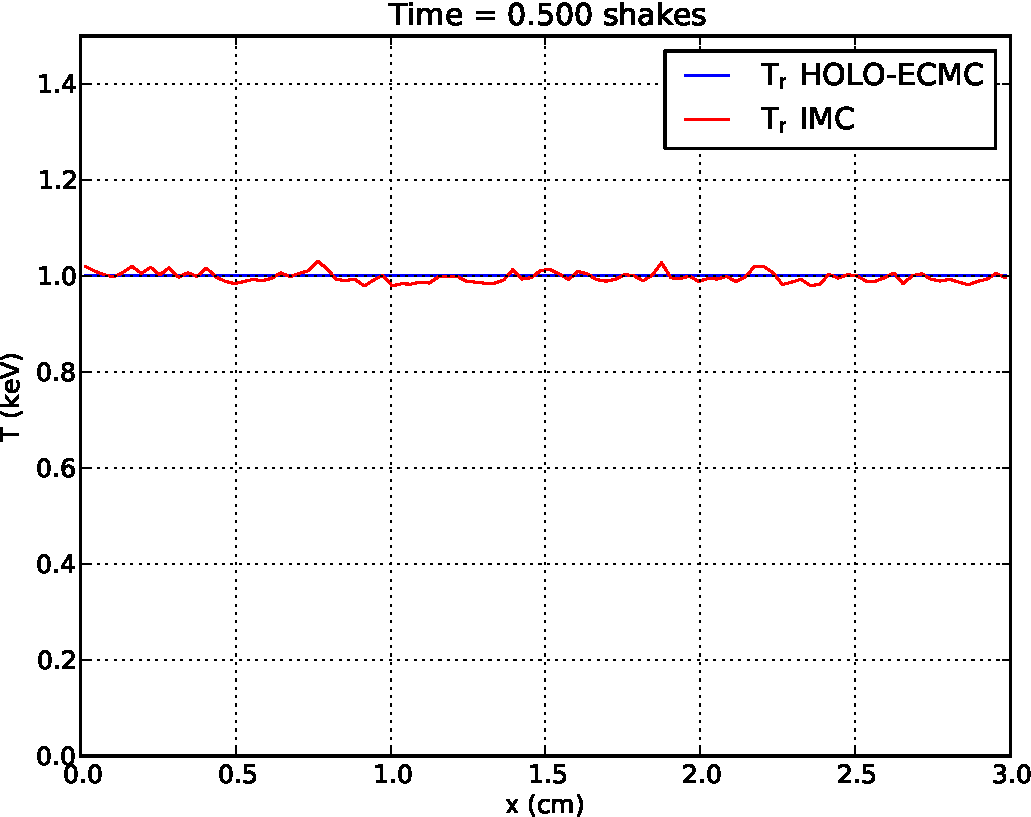
\includegraphics[width=0.6\textwidth]{constant.pdf}
   \caption{\label{constant_fig} Comparison of IMC and HOLO-ECMC results for
       an equilibrium solution.}
\end{figure}


\Subsection{Two Material Problem}

This problem consists of an optically thin and an optically thick material region,
with constant cross sections.  This problem demonstrates the utility of the
hybrid method in both the streaming (left) and diffuse (right) regions of the domain.  The material properties are given in
Table~\ref{two_mat_props}.  Initially the radiation and material energies are in
equilibrium at a temperature of 0.05 keV.  An isotropic incident intensity of 0.500 keV
is applied at $x=0$ at $t=0$; the incident intensity on the right boundary is 0.05
keV.  The simulation was ran for 5 shakes with a
time step size of 0.001 shakes.  

Fig.~\ref{twomat_quick} compares the HOLO, IMC, and diffusion computed radiation temperatures at $t=0.010$ sh.  Both curves plot the cell-wise averages rather than the LD representation.  At this point in the simulation, the radiation is in the optically thin region of the problem, so the diffusion solution has propagated too quickly.  The IMC and HOLO methods agree well.  Fig~\ref{twomat_full} compares the IMC and HOLO radiation temperature profiles at the end of the simulation.  The wave fronts show good agreement.  
These results were computed using the lumping-equivalent discretization for the LO solver, noting that this is not consistent with the HO solver.  A consistent discretization in the HO solver would likely produce a more accurate solution. 
\begin{table}[htb]
    \begin{center}
        \begin{tabular}{|c|cc|}  \cline{2-3}
            \multicolumn{1}{c|}{}   & $x \in [0,0.5)$ cm & $x \in [0.5,1.0]$ cm   \\ \hline
            $\sigma_a$ (cm$^-1$)  & 0.2 & 2000 \\
            $\rho$ (g cm$^-3$) & 0.03 & 10.0 \\
            $c_v$ (jks/keV-g) & $0.1$ & $0.1$ \\ \hline
        \end{tabular}
        \caption{Two material problem properties \label{two_mat_props}}
    \end{center}
\end{table}
\begin{figure}
\centering
    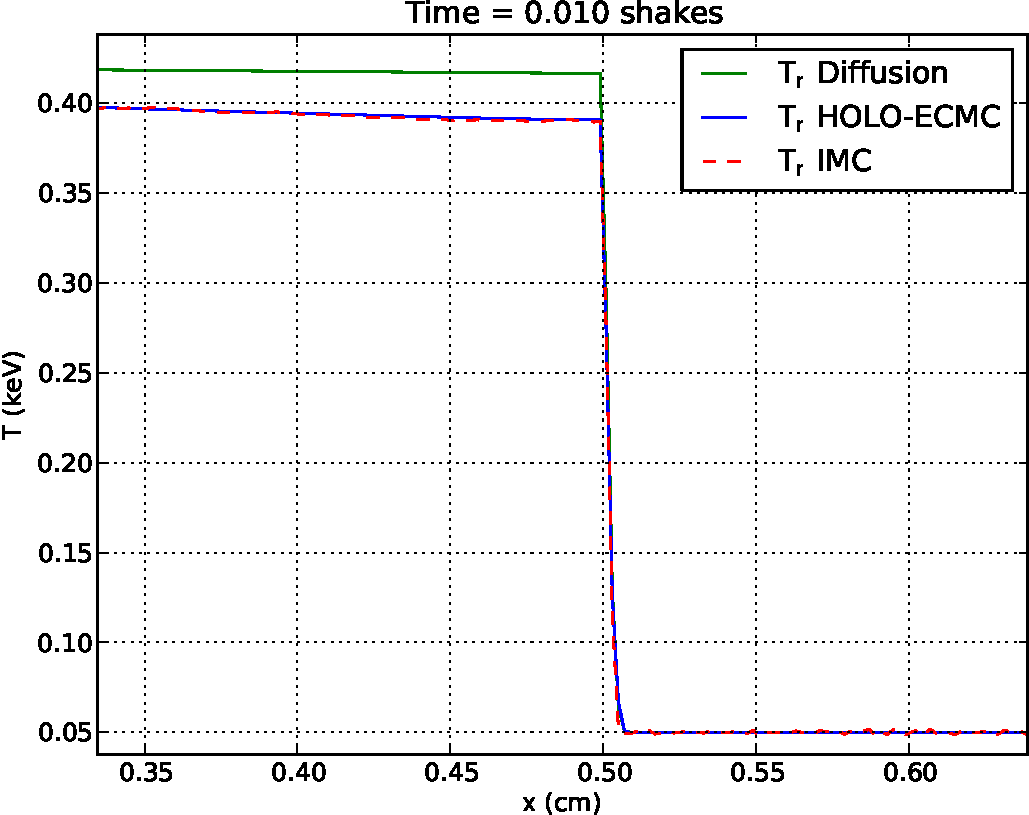
\includegraphics[width=0.59\textwidth]{twomat_holo_quick.pdf}
    \caption{Comparison of radiation temperatures for HOLO-ECMC, IMC, and diffusion for two material problem after 10 time steps. \label{twomat_quick}}
\end{figure}
    \begin{figure}
    \centering
    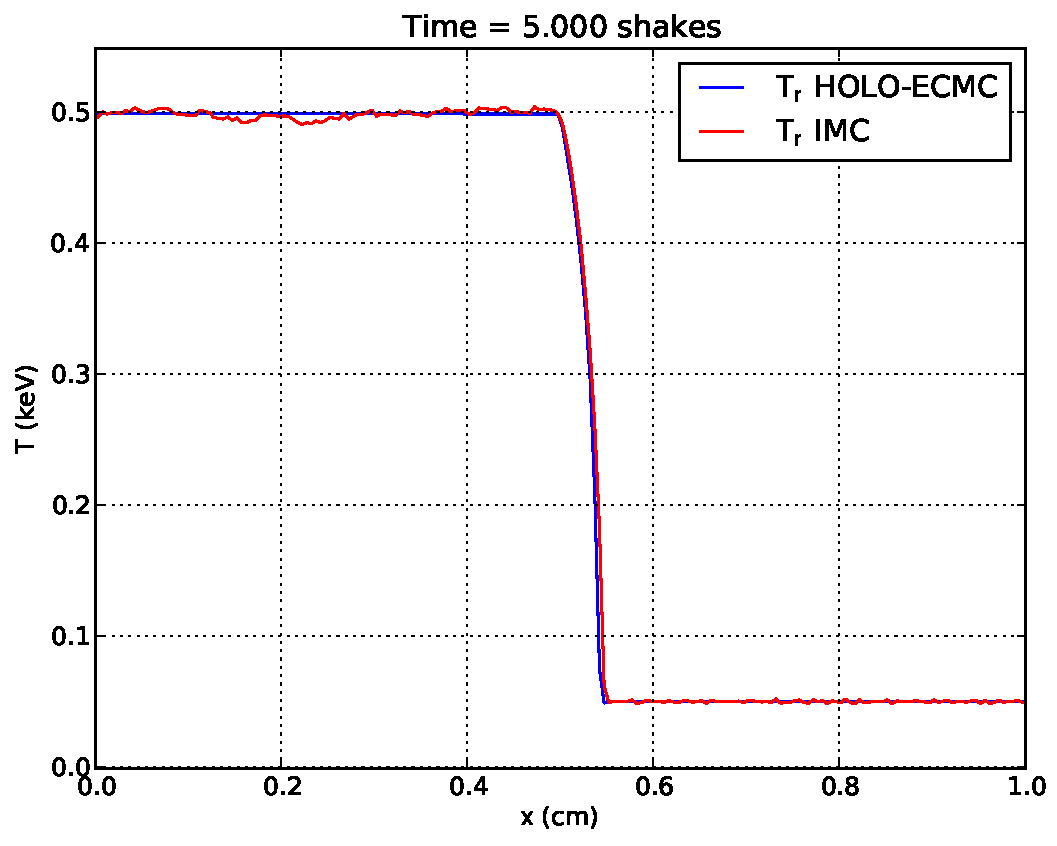
\includegraphics[width=0.59\textwidth]{twomat_full.pdf}
    \caption{Radiation temperature profiles for two material problem after 5 shakes.\label{twomat_full}}
    \end{figure}

\Subsection{Marshak Wave}

For this problem, initially the radiation and material energies are in equilibrium at 2.5E-05 keV.   An isotropic incident intensity of 0.150 keV
is applied at $x=0$ at $t=0$; the incident intensity on the right boundary is 2.5E-05 keV.  The material properties are $\rho = 1$ g cm$^-3$ and $c_v = 0.013784$ jks/keV-g. The absorption cross section varies as
\begin{equation}
\sigma(T) = \frac{0.001 \rho}{T^3},
\end{equation}
which introduces a strong non-linearity into the problem.   The simulation was ran for 5 shakes with a
time step size of 0.001 shakes. 

Fig.~\ref{marshak_holo_ld} compares the cell average radiation temperatures for the IMC and HOLO methods.  The radiation wave front is significantly farther ahead in the HOLO method.  Simluations with a refined mesh and time step did not remove this discrepancy, and the IMC solution did not move much.  This suggest that the fact that IMC lags opacities is not the cause of the difference.  There are a couple notable issues that could be the cause of the discrepancy.  Although the averages are positive, the LD representation of the intensity leads to engativites near the steep wave front.  The negativities lead to poor consistency terms.  Additionally, histories with large negative weights in the wave-front region enter the equilibrium cells to the right and cause poor statistics due to the thick cross section.  This leads to consistency terms that are unphysical ($\mom{\mu} \notin [ -1, 1]$) in cells near the wave front.  In these cells diffusion equivalent  parameters are used for the parameters that are bad.  The diffusion approximation near the wave front ultimately leads to a faster wave speed.  There are a couple ideas discussed in future work for correcting the bad statistics on the right side of the wave front.

Fig.~\ref{blading} plots the LD representation of the material and radiation energies (in this figure the negativities in the radiation are plotted as zero, but due exist at the wave front).  The steep, unphysical gradients in the material temperature distribution are a result of using cell-wise constant cross sections.  More accurate, spatially varying cross sections will be implemented in future work.  

To correct issues introduced into the LO solver by negativities in the radiation equation, the lumped-equivalent spatial discretization discussed previously was implemented for the LO solver.  The HO solver was left as LD in space in angle.  Thus, the LO discretization preserves the $L$ and $R$ moments of the HO solution, but does not use a consistent outflow.  Results with this alternative LO discretization are displayed in Fig.~\ref{lumped_marshak}.  The wave speeds are much closer, but there is still a noticeable discrepancy.   The first and easiest method for resolving this issue would be to implement a similar strictly positive discretization in the HO solver to ensure consistency.  This will likely resolve some of the issues with noise resulting in bad consistency terms.
    \begin{figure}
    \centering
    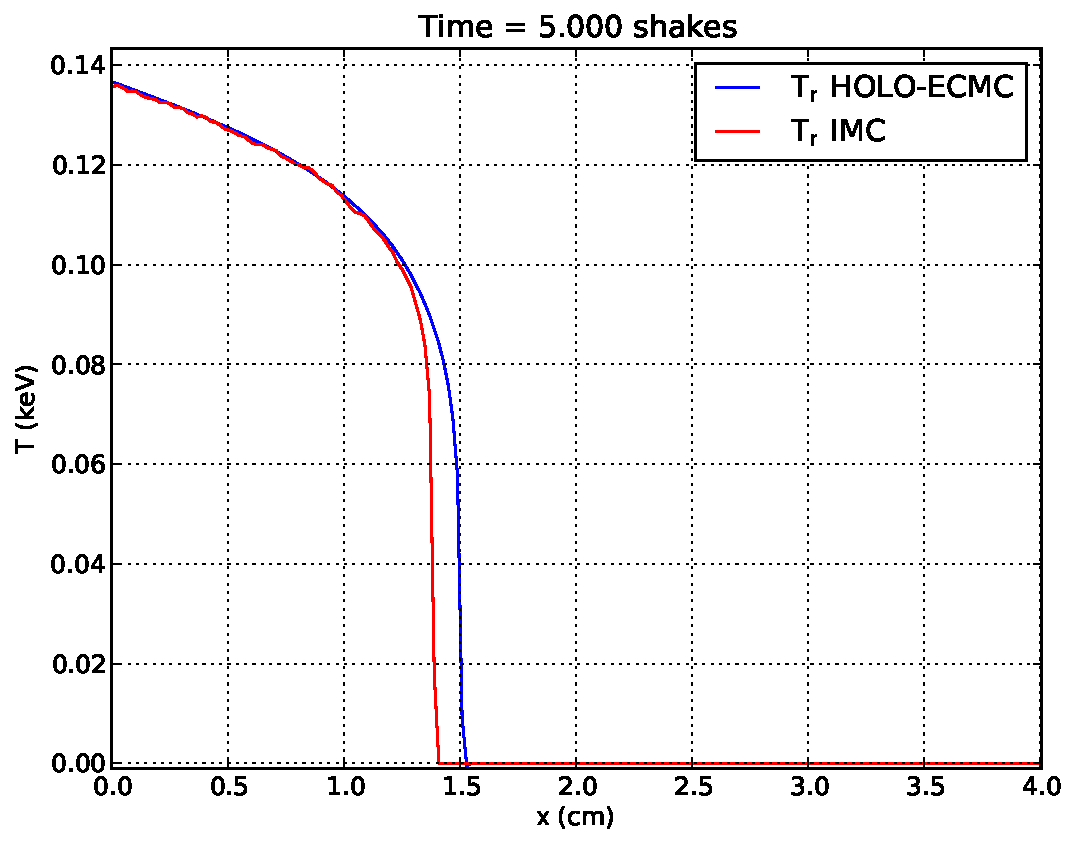
\includegraphics[width=0.59\textwidth]{marshak_holo_ld.pdf}
    \caption{\label{marshak_holo_ld} Comparsion of cell-averaged radiation temperatures for Marshak wave problem.}
    \end{figure}
    \begin{figure}
        \centering
    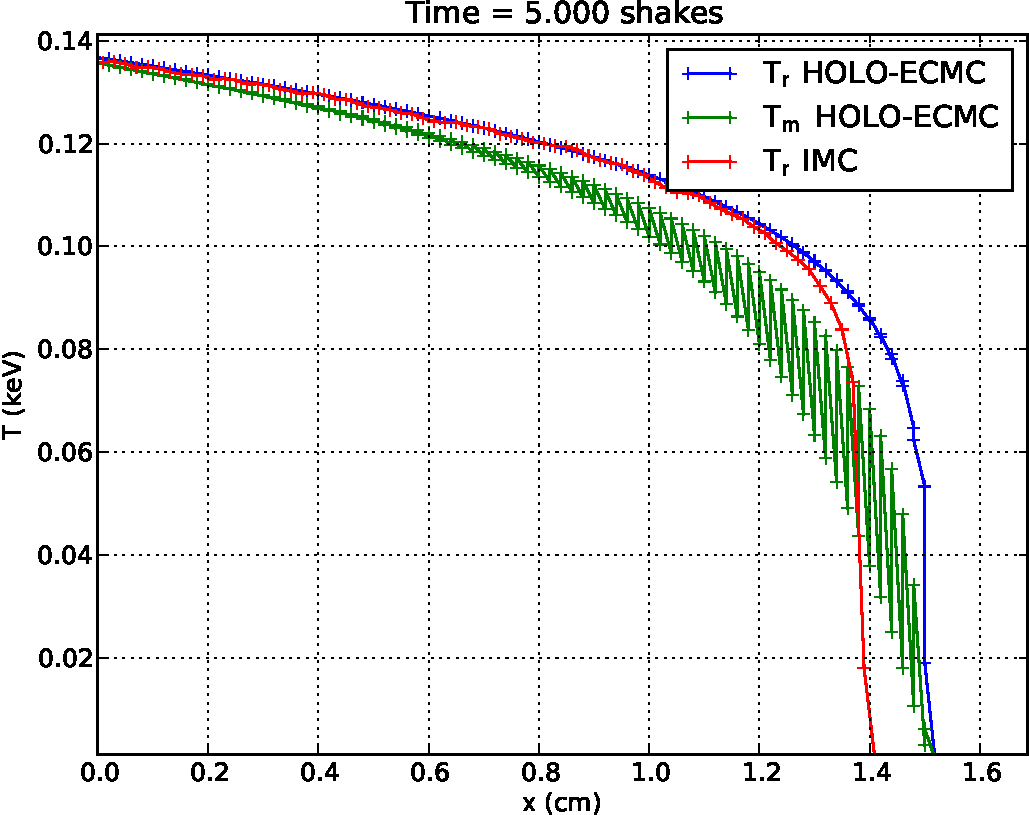
\includegraphics[width=0.59\textwidth]{blading.pdf}
        \caption{\label{blading} LD representation of material and radiation energy temperatures for HOLO, as compared to cell averages for IMC, for Marshak wave problem.}
    \end{figure}
    \begin{figure}
        \centering
    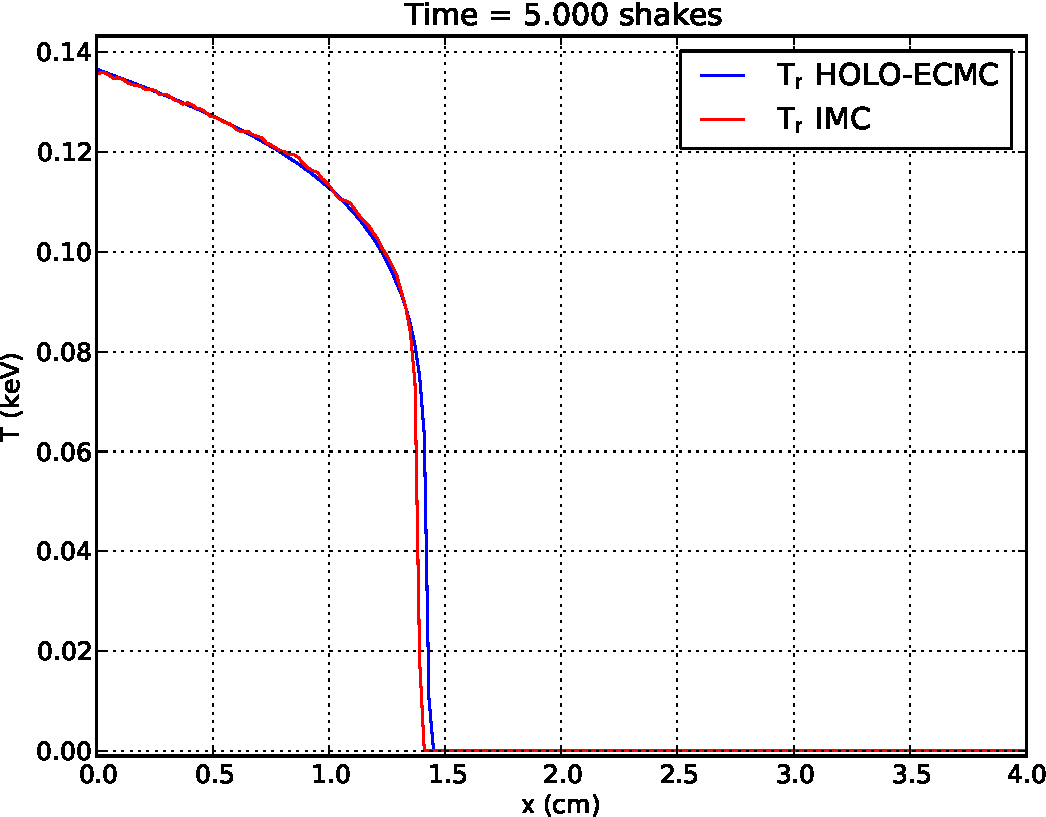
\includegraphics[width=0.59\textwidth]{marshak_holo_lumped.pdf}
        \caption{\label{lumped_marshak} Marshak wave problem with lumped-equivalentLD spatial representation for  LO
        solver.}
    \end{figure}

\Section{Conclusions}

We have been able to reproduce the IMC solutions for certain problems using a new HOLO method.  The primary difficulty is in the speed of wave fronts for the Marshak wave problem.  The LO solver resolves the non-linearities in the equations resulting in a fully implicit time discretization.  The ECMC approach, with initial guesses based on the previous radiation intensity, results in efficient reduction of statistical error and allows for particles to be distributed to largely varying regions of the problem.  Analytic transport benchmark results are
needed for a direct comparison of the accuracy between the HOLO and IMC methods.  However, most of
the transport benchmarks utilize reflective boundary conditions.
Reflective boundary conditions have been successfully implemented in the LO solver,
but have not yet been successfully implemented in the HO solver.  An explanation of the
difficulties with reflective boundary conditions is detailed in the Appendix.  Once
the reflective boundary conditions are correctly implemented, a comparison of the
accuracy of the two methods can be made.

Other future work will include continuous energy deposition tallies as a form of variance reduction.  Also, a strictly positive spatial discretization in the HO system will be implemented.  If this does not resolve issues with statistical noise, a form of cell-wise error filtering will be implemented.  With the exception of the first batch, it is not expected that the relative error in a cell should be less than 1.  If this is the case, then it is likely due to a bad MC estimate.  These cases could be rejected and the previous estimate of the intensity in that cell used for the next calculation, or a damped version of the change could be used.    Long term work will include adding the ability to handle opacities that vary as lLD with temperature in space.  A multigroup formulation will be explored, before extending to multiple spatial dimensions.

\bibliography{references}
\bibliographystyle{unsrt}    
\clearpage

\appendix

\Section{Derivation of the LO Equations for Neutronics}
\label{sec:lo}
The basic LO equations are derived for the simple case of a fixed source problem with
scattering.  The differences for TRT problems will be in the external source term,
including the angular intensity from the previous time step, and addition of the material energy
equation. The HOLO iteration indices are added at the end. Starting with the slab transport equation (with constant cross sections
for simplicity)
\begin{equation}
\mu \pderiv{\psi}{x} + \sigma_t \psi(x,\mu) = \frac{\sigma_s}{2} \phi + \frac{q}{2}
\end{equation}
where $\phi=\int_{-1}^1 \psi \;\d \mu$ is the scalar flux and $q$ here is some fixed
external source (unrelated to the $q$ in other sections).  The spatial moments are
taken over each spatial cell $i$: $x\in[x_{i-1/2},x_{i+1/2}]$ using the usual hat
functions, e.g., for the left basis
\begin{equation}
b_L(x) = \frac{x_{i+1/2} - x}{h_i}
\end{equation}
with spatial moment defined as
\begin{equation}
\mom{\cdot}_{L,i} = \frac{2}{h_i} \int_{x_{i-1/2}}^{\xr} b_L(x) (\cdot) \d x,
\end{equation}
where $h_i$ is the width of the spatial element.
Application of the above operator to the transport equation, after integrating by parts and some manipulation, produces
\begin{equation}\label{left}
-2\mu \psi_{i-1/2} + \mu \left( \mom{\psi}_{L,i} + \mom\psi_{R,i} \right) + \sigma_t h_i \mom{\psi}_{L,i} = \sigma_s h_i \mom{\phi}_{L,i} + h_i \mom{q}_{L,i}
\end{equation}
where $\psi_{i-1/2}$ is the left face value of the angular flux. An important step in the above manipulation is the relation
\begin{equation}
\psi_{a,i} = \frac{1}{h}\int_0^1 \psi(x) \d x = \frac{1}{2} \left(\mom{\psi}_{L,i} + \mom{\psi}_{R,i} \right) 
\end{equation}
because $b_L(x) + b_R(x) =1 $.  

 Since the external
source is assumed to belong in the trial space, that moment can be analytically
evaluated as
\begin{equation}\label{left_mom}
\mom{q}_{L,i} = \frac{2}{3} q_{i-1/2} + \frac{1}{3} q_{i+1/2}.
\end{equation}
Half range moments are then taken, defining
\begin{equation}
\phi^+ = \int_0^1 \psi \d \mu.
\end{equation}
Thus, $\phi = \phi^- + \phi ^+$.
The positive half range moment of Eq.~\eqref{left}, with substitution for $\phi$, produces
\begin{equation}
-2 \int_0^1\mu \psi_{i-1/2} \d \mu + \int_0^1\left[\mu \mom{\psi}_{L,i} +  \mu \mom\psi_{R,i} \right] \d \mu + \sigma_t h_i \mom{\phi}_{L,i}^+ = \sigma_s h_i \left( \mom{\phi}_{L,i}^+ + \mom\phi_{L,i}^-\right) + h_i \mom{q}_{L,i}
\end{equation}
Each term is divided and multiplied by the corresponding integrals over half range
and spatial moment to produce averages of $\mu$ where needed. For example
\begin{equation}\displaystyle 
\mom{{\mu}}_{L,i}^+ \mom{\phi}_{L,i}^+ = \left( \frac{\displaystyle 
\frac{2}{h_i} \int\limits_0^1 \int\limits_\xl^\xr \mu \, b_L(x) \psi(x,\mu) \d \mu \d x } 
{\displaystyle \frac{2}{h_i} \int\limits_0^1 \int\limits_\xl^\xr \, b_L(x) \psi(x,\mu) \d \mu \d x } \right)
* \displaystyle \frac{2}{h_i} \int\limits_0^1 \int\limits_\xl^\xr \, b_L(x) \psi(x,\mu) \d \mu \d x 
\end{equation}
Applying to the streaming terms produces the final equation
\begin{equation}
-2{\mu}_{i-1/2}^+ \phi_{i-1/2}^+ + \mom {\mu}_{L,i}^+ \mom{\phi}_{L,i}^+ +  \mom\mu_{R,i}^+
\mom{\phi}_{R,i}^+ + \sigma_t h_i \mom{\phi}_{L,i}^+ =  \sigma_s h_i \left( \mom{\phi}_{L,i}^+ +
\mom\phi_{L,i}^-\right) + h_i \mom{q}_{L,i},
\end{equation}
where $\mu_{i-1/2}^+$ indicates the positive half-range average of $\mu$ over the
$\il$ face.
Similarly, the $R$ moment equation can be shown to be
\begin{equation}
2{\mu}_{i+1/2}^+ \phi_{i+1/2}^+ - \left( \mom\mu_{L,i}^+ \mom{\phi}_{L,i}^+ +  \mom\mu_{R,i}^+ \mom{\phi}_{R,i}^+ \right) + \sigma_t h_i \mom{\phi}_{R,i}^+ =  \sigma_s h_i \left( \mom{\phi}_{R,i}^+ + \mom\phi_{R,i}^-\right) + h_i \mom{q}_{R,i}
\end{equation}
The $-$ direction equations are essentially the same with $+ \rightarrow -$ (there is
a difference in the upwinding and extrapolated face terms, explained below). The two
equations for negative flow are
\begin{align}
-2{\mu}_{i-1/2}^- \phi_{i-1/2}^- + \mom {\mu}_{L,i}^- \mom{\phi}_{L,i}^- +  \mom\mu_{R,i}^-
\mom{\phi}_{R,i}^- + \sigma_t h_i \mom{\phi}_{L,i}^- &=  \sigma_s h_i \left( \mom{\phi}_{L,i}^+ +
\mom\phi_{L,i}^-\right) + h_i \mom{q}_{L,i},
\\
2{\mu}_{i+1/2}^- \phi_{i+1/2}^- - \left( \mom\mu_{L,i}^- \mom{\phi}_{L,i}^- +  \mom\mu_{R,i}^-
\mom{\phi}_{R,i}^- \right) + \sigma_t h_i \mom{\phi}_{R,i}^- &=  \sigma_s h_i \left( \mom{\phi}_{R,i}^+ + \mom\phi_{R,i}^-\right) + h_i \mom{q}_{R,i} .
\end{align}
Here it is noted that the ${\mu}^-$ averages involve integrals of the form
$\int_{-1}^0 \mu \psi(\mu) \d \mu$.  This is not consistent with the usual definition
of $j^-= \int_{-1}^0 |\mu|\psi(\mu) \d\mu$, differing by a factor of $-1$.

\Subsection{Angular Consistency with the HO Solver}
\label{consist}

The above equations represent four equations, for each cell, for the unknowns $\mom{\phi}_{L,i}^+$,
$\mom{\phi}_{R,i}^+$, $\mom{\phi}_{L,i}^-$, and $\mom{\phi}_{R,i}^-$.  These unknowns can
be used to construct an LD representation of the scalar flux over each cell.
Again, these coupled equations are exact; no discretization has been introduced
yet.  However, the $\mom{\mu}$ parameters are not known a priori.  These $\mu$
parameters are lagged, i.e., in the HOLO context from the HO solution at $k+1/2$.  The parameters are based on the previous estimate of these parameters computed
by the HO solution.  For example, for the $L$ moment equation and positive flow the
final LO equation becomes
\begin{multline}
  -2{\mu}_{i-1/2}^{+,k+1/2} \phi_{i-1/2}^{+,k+1} + \mom {\mu}_{L,i}^{+,k+1/2}
  \mom{\phi}_{L,i}^{+,k+1}
  +  \mom\mu_{R,i}^{+,k+1/2}
  \mom{\phi}_{R,i}^{+,k+1} + \\  \sigma_t h_i \mom{\phi}_{L,i}^{+,k+1}  =  \sigma_s
  h_i \left( \mom{\phi}_{L,i}^{+,k+1} +
  \mom\phi_{L,i}^{-,k+1}\right) + h_i \mom{q}_{L,i},
\end{multline}
where the average $\mu^{k+1/2}$ parameters are estimated based on the previous HO solution
for the angular flux, e.g.,
\begin{equation}\displaystyle 
\mom{{\mu}}_{L,i}^{+,k+1/2} = \frac{\displaystyle 
  \frac{2}{h_i} \int\limits_0^1 \int\limits_\xl^\xr \mu \, b_L(x) \psi^{k+1/2}(x,\mu) \d \mu \d x } 
  {\displaystyle \frac{2}{h_i} \int\limits_0^1 \int\limits_\xl^\xr \, b_L(x)
\psi^{k+1/2}(x,\mu) \d \mu \d x } 
\end{equation}
Because the HO solution produces an accurate LD functional form of the angular flux
everywhere,
the above equations can be evaluated directly.  As a result of the low statistical error produced by ECMC, the accuracy of $\psi^{HO}(x,\mu)$
is primarily dependent upon the accuracy of the LD representation of sources estimated from the
previous LO solution.  As the HO and LO solution are converged to the consistent solution,
the LO system becomes exact to the precision of the convergence between the two solutions. 
For an initial approximation to the LO solution, all average $\mu$ parameters are
set to $\pm 1/\sqrt{3}$ as appropriate, yielding a solution equivalent to diffusion
with Mark boundary conditions (S$_2$).

\Subsection{Spatial Consistency with the HO Solver}

To close the LO system spatially, for stability, the usual LD upwinding
approximation is used.  For example, for positive flow, the $\mu_{i-1/2}$ and $\phi_{i-1/2}$
terms are upwinded from the previous cell or boundary condition.  The $R$ moment equation has no upwinded term for positive flow, but
the right face value is extrapolated based on the $L$ and $R$ basis moments.
Boundary conditions are represented exactly because $\mu_{i-1/2}^+
\phi_{i-1/2}^+ = j_{i-1/2}^+$, the incident half range current.  Because the HO
solver uses an LD representation in space, the spatial closures are inherently
consistent.  

The spatial relation between the outgoing face values of the flux to the volumetric
moments could be estimated accurately from the HO solver, e.g., for positive flow
\begin{equation}
\phi^+_{i+1/2} = \alpha^+ \mom{\phi}_R^+ + (1-\alpha^+) \mom{\phi}_L^+ 
\end{equation}
where $\alpha^+$ is computed from the HO solution of the above equations.  This
would produce a more exact spatial closure (there is still truncation error from the upwinding
approximation).  However, the outgoing face values are not in our trial space currently for the HO solver, so
accurate estimation of such tallies would not be readily obtained.  Since the
HO solution is spatially LD, the value of $\alpha^\pm$ is 2 over each cell, producing a LD closure for the LO
system. 

\Section{Alternative Temperature Linearization}
\label{alt}


\Section{ECMC Reflective Boundary Conditions}

Typical incident intensity boundary conditions are straightforward to handle in the
residual equation for the HO ECMC system. However, reflective boundary conditions require special attention
in the HO system that is atypical for MC simulations.  For the residual calculations, 
a typical incident intensity is sourced is treated via vacuum boundary conditions with an effective
residual boundary source.  The energy is sourced on the boundary as an upwinded term in the computation of
the residual delta source term $-\mu \pderiv{\tilde{I_b}^{n+1}}{x}$ evaluated on the
boundary face.
In the case of reflective boundaries, particle histories are specularly reflected as
in standard MC, i.e., $\tilde{\epsilon_b}(\mu) = \tilde{\epsilon_b}{-\mu}$.  However,
an additional source term must be added because the value of $I(\mu)=I(\-mu)$ on the
boundary is not in general equivalent to the LD extrapolated value of $I$ on teh
boundary. This adds a face source term as with the incident intensity boundary
condition, so an
estimate of $I_b(\mu)$ is required.  This can be computed on a cell-wise basis based
on the LD extrapolated outflows, i.e., $I_b(-\mu)$, in the cells that match $-\mu$.
This may be difficult as a result of the different.  As an alternative, the outgoing
intensity can be estimated via a face tally.  This effectively changes the trial
space in outgoing cells to have an upwinded inflow, a linear representation with in
the cell, and then a fixed outflow estimated based on all particle histories that
cross that cell.  Although this will generally not be as accurate, implementation
should prove much easier than estimating the inflow based on the outflows due to the
varying refinement levels in the cells.


\Section{SECOND OR SUBSEQUENT MAJOR HEADING} 
\label{sec:first}

This is Section~\ref{sec:first}. It is followed by a Subsection, that is, 
\ref{sec:second}. For this class file you must use the 
\texttt{$\backslash$Section\{\}} to denote sections (note the capital ``S'').  
The style for subsection titles and all text in this template is defined in 
the {\it mc2013.cls} file.  Make sure to avoid widow/orphan lines.


\Subsection{Subsection Title: First Character of Each Non-trivial Word is 
Uppercase} 
\label{sec:second}

Double-space before and after secondary titles is automatic.  Figures and 
tables should appear as close as possible to where they are first
cited, e.g., Fig. \ref{fig:amdahl}, in the text.  Figures are numbered in 
Arabic numerals, with the caption centered below the figure, in 
{\bf boldface}.
  
Triple-space before the figure, and after the figure caption.

%
\vspace{16pt}
\begin{figure}[!htb]
\begin{spacing}{1.0}
\centering
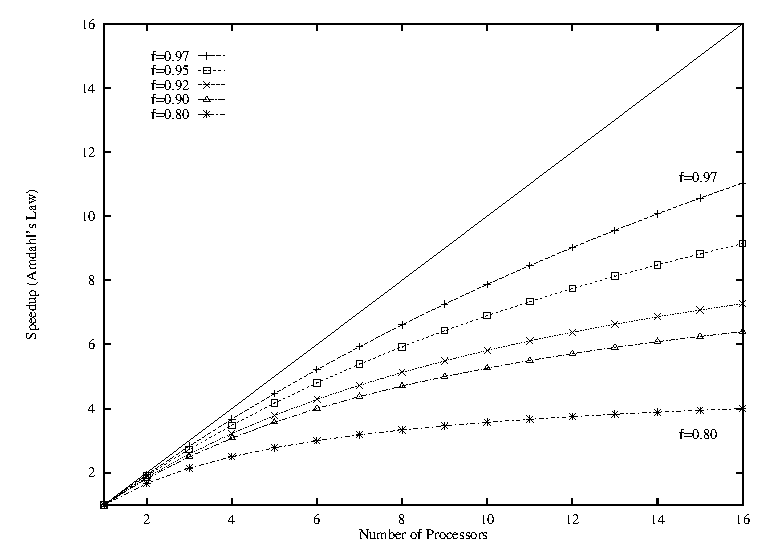
\includegraphics[scale=0.60]{./figure.eps}
\caption{\bf Speedup vs Number of Processors for Varying Parallelizable 
Fractions in Order to See a Multiple Line Caption} 
\label{fig:amdahl}
\end{spacing}
\end{figure}
\vspace{16pt}
%

When importing figures or any graphical image please verify two things:
\begin{itemize}
\item Any number, text or symbol is in Times font and is not smaller than 
    10-point after reduction to the actual window in your paper
\item That is can be translated into PDF
\end{itemize}


Equations, such as Eq. (\ref{sample_equation}), should be centered and 
sequentially numbered to the flush right of the formula.
\begin{equation}
\label{sample_equation}
Speedup\ =\ {1 \over{{f \over {p}} + (1-f)}}
\end{equation}
The continuation of a paragraph after an equation should not be indented.  
All paragraphs, as well as section or subsection headings, are separated by 
just one single empty line.


\Subsubsection{Sub-section level and lower: only first character uppercase}

See Table \ref{table:example} for a sample table.  The tabls package is
recommended for improved row and column spacing.  Notice the caption appears 
above the table by setting the \texttt{$\backslash$caption} command immediately 
after the \texttt{$\backslash$begin\{table\}}. Tables are numbered in Roman 
numerals, with the caption centered above the table, in {\bf boldface}.  
Triple-space before and after the table.

\vspace{16pt}
\begin{table}[!htb]
\centering
\caption{\bf Parallel Performance for the Sample Problem}
\label{table:example} 
\vspace{14pt}
\begin{tabular}{||r||c|c|c||} \hline \hline
 \multicolumn{1}{||c||}{Number of} &
 \multicolumn{1}{c|}{Wall-Clock} &
 \multicolumn{1}{c|}{Speedup} &
 \multicolumn{1}{c||}{Efficiency} \\
 \multicolumn{1}{||c||}{Processors} &
 \multicolumn{1}{c|}{Time$^{a}$ (min)} &
 \multicolumn{1}{c|}{(T$_{s}$/T$_{p}$)} &
 \multicolumn{1}{c||}{(\%)} \\ \hline\hline
\ 1 &  100.0 & \ ---    & ---  \\ \hline
\ 2 &   52.6 & \ 1.9    & 95.0 \\ \hline \hline
\end{tabular}
\end{table}
\vspace{16pt}


\Section{CONCLUSIONS}

Present your summary and conclusions here.


\section*{ACKNOWLEDGEMENTS}

This research was performed, in part, using funding received from the DOE Office of Nuclear
Energy's Nuclear Energy University Programs.


%\Section*{REFERENCES}
\setlength{\baselineskip}{12pt}
\begin{thebibliography}{300}
\bibitem{journal} B. Author(s), ``Title,'' {\it Journal Name in Italic}, 
          {\bf Volume in Bold}, pp. 34-89 (19xx).
\bibitem{willert} J. Willert, C.T. Kelly, D.A. Knoll, and H. Park,
         ``A Hybrid Approach to the Neutron Transport k-Eigenvalue Problem using
         NDA-based Algorithms,'' {\it M\&C}, Sun Valley, ID, May 5-9 (2013).
\bibitem{park} H. Park, J.D. Densmore, A.B. Wollaber, D.A. Knoll and  R.M. Ramenzahn,
                ``Monte Carlo Solution Methods in a Moment-Based Scale-Bridging
                Algoirthm for Thermal Radiative Transfer Problems: Comparison with
                Fleck and Cummings,'' {\it M\&C}, Sun Valley, ID, May 5-9 (2013).
\bibitem{book} E. F. Author, {\it Book Title in Italic}, Publisher, City \&
          Country (19xx). 
\bibitem{website} ``Spallation Neutron Source: The next-generation 
          neutron-scattering facility in the United States,'' 
          http://www.sns.gov/documentation/sns\_brochure.pdf (2002).
\end{thebibliography}

\end{document}


